\section{System Overview}

Though it may appear trivial at first, the broad scope of the design space of this project meant making difficult design decisions where there was often no clear answer.  The first major decision was determining the approach used to reduce the swapping time.  Inspired by the battery connectors in some wearable devices, a hot swapping connector design was chosen.  Hot swapping refers to the ability to connect or disconnect a peripheral, in this case a guitar pedal, without needing to perform any special preparatory actions such as turning off the power.  This type of design unites a physical action of inserting or removing a pedal into a system with the electrical switching actions required to actually perform the hot swapping.

With this decision made, the high level design of the hot swapping device was considered.  To be able to insert a pedal into the signal chain at any time meant that the solution required a main signal control device, which acts as a "meta pedal", connected between the guitar and an amplifier.  When the hot swapping device is not activated, the guitar signal is connected directly to the amplifier.  When the hot swapping action occurs, the signal is routed through the hot swapping connector to the pedal and back, allowing the pedal to be inserted into the signal chain between the guitar and amplifier.

This required standardizing the interface between the guitar pedal and the device.  Data collected during a site visit to a Guitar Center retail location demonstrated the plethora of effects pedals available at a standard brick-and-mortar store.  These 150 pedals represent a good mix of products, from mass market production units such as the Boss DS-1 to high quality and expensive effects like Eventide’s H9. While the major manufacturers like Boss, MXR, and Electro Harmonix have narrowed their form factors down to a handful of types each, there is no standardization across producers on features important for this project, including the dimensions of the enclosure, the location and orientation of the signal and power jacks, the location of the screws used to hold the pedal’s bottom plates. Though most products use the de facto standard 9 VDC, center negative power supply connected with a 2.1 mm plug, this too has variations in some cases. All of these variations complicate standardizing a form that can easily be hot swapped.  A universal adapter was designed to connect the pedal to the hot swapping device.

On a high level, the design process focused on ease of use and intuition for the user over any other considerations where possible, which explains the preference for this tactile and tangible hot swapping method over a programmable switching device, for instance.  The push for simplicity has led to some increases in design complexity, including the need to automatically detect when a hot swapping event occurs rather than include a separate user controlled switch.

In order for a user to be able to test multiple effects, multiple hot swapping devices were included in the device.  An internal signal routing system was also designed to facilitate testing pedals in different routing configurations including series, parallel, feedback, and various combinations of these.  Finally, a user interface was designed to control this internal signal routing.

Because of the repetition present in the device, it was designed as a modular system to simplify design, fabrication, and evaluation.  Figures \ref{fig:system_block} and \ref{fig:module_block} show a hierarchical block diagram of the system.  The system level diagram shows three modules were used for the full implementation of the system, with only audio passing between them.  The same $24VDC$ power input was passed to each module.  The module level diagram shows the major constituent parts of each module.  The design and function of each of these will be discussed in the remainder of this chapter.

\insertimage{0.95}{FinalImages/SystemBlock_white.jpg}{System level of hierarchical block diagram.  This shows the modular design of the device.  The legend in the upper right shows that power is indicated in red, audio signal in black, and control signals in green, with the direction of the arrow indicating data direction.  Note that no control signals pass between the modules, making design and debugging simple.  The signal and power I/O for the device are passed on to the modules.}{fig:system_block}

\insertimage{0.95}{FinalImages/ModuleBlock_white.jpg}{Module level block diagram showing the contents of each module.  As in Figure \ref{fig:system_block}, power is indicated in red, audio signal in black, and control signals in green, with the direction of the arrow indicating data direction.  In principle, each module contains a pair of hot swap devices consisting of the hot swap connector, DPDT switching element, and adjustable voltage regulator.  The module also contains an internal signal routing mechanism consisting of two mixers and a user interface, as well as all necessary voltage regulators required to step down the 24V input for all these circuits.}{fig:module_block}

\section{Design Decisions}
	\subsection{Universal Adapter}
	

	Because of the large variety of guitar pedal shapes, they are not by themselves suitable for hot swapping in and out of a fixed receiving unit. A universal adapter was designed to interface between the pedal's I/O and the hot swapping connector.  The required attributes for this adapter include a way to mechanically mount a pedal, a way to connect to the pedal's I/O, and a way to connect to the hot swapping connector.  The last requirement means that there must be exposed electrodes with which the corresponding electrodes on the main device can make electrical connection.  It also includes a method to physically align these electrodes when the hot swap device is active.  None of these requirement suggest a need for much vertical height, so this universal adapter will in general come in the form a base plate on which the pedal sits.  Because of this, "plate" is used to refer to this universal adapter throughout the rest of this document.  

		\subsubsection{Pedal-Plate Mounting}

		The thin and flat nature of the universal adapter plate allows the plate itself to be used as part of fastening the pedal.  Holes and slots cut into the plate which allow screws to pass open up several options for mounting a pedal.  Because of its simplicity, the most attractive option was to reuse the screws that hold in the pedal's bottom cover.  As most pedal enclosures have bottom covers held on by four screws, one in each corner, reusing two screws in opposite corners to pass through the plate allows the cover to remain in place while still resulting in a good mechanical connection between the pedal and the plate.  However, because a non-trivial number of effects pedal enclosures have fewer bottom plate screws, or none at all, this method is not completely universal.

		To accommodate pedals that do not have the common four-screw bottom plate, a clamping mechanism can be used to modify the method described above.  Instead of reusing pedal's bottom plate screws, a clamp in the shape of a corner bracket is placed over the top corner of the pedal, and a screw is again passed through the plate used to tighten the corner clamp down, securing the pedal along with it.  This solution allows the same type of holes and slots used with the direct bottom cover screw method.  The clamp should be padded to prevent damage to the product.  Although this augmentation to the bottom cover screw method would help to increase compatibility, it was not explored further due to time constraints.

		The advantage of both of these methods is that they are easily reversible and have no lasting effects on the appearance or function of the product.  However, if neither of the above attachment methods was adequate, Velcro could also be used to attach the pedal to the plate, as is common with permanent pedalboard setups.  However, this can leave a residue on the product so it is less desirable.

		\subsubsection{Plate Size}

		The position and dimension of the slots and holes required for the through-screw methods of mechanical attachment mentioned above must be positioned to allow alignment with the pedal's bottom cover screw holes.  Because this varies with the exact geometry of the enclosure, these holes should allow for adjustment.  Slots were chosen over holes as the primary mating location because of their allowance for adjustment along an axis.  To determine the exact shape of the slots, measurements of the physical dimensions of pedals at Guitar Center were taken, to determine a guideline to estimate the relative position of the bottom plate screw holes compared to the outer dimensions of the enclosure.  Based on the measurements taken, the distance between screws in any direction is typically 90\% to 95\% of the outer length of the enclosure in that dimension.  Using this, the physical outer dimensions of all of the pedals cataloged at Guitar Center were recorded from each pedal's user manual.

		Because only two screws located on opposite corners of the pedal are used to attach the pedal to the plate, a line can always be draw through both of them\footnote{This is very trivial}.  Therefore, when designing the mounting slots on the plate it is sufficient only to consider the length of this line segment connecting the two screw locations.  Variations in the aspect ratio of the enclosure (width to height) can be dealt with via small rotations.  The data collected from Guitar Center stock was used to actually design the minimum and maximum screw-hole-distances that must be covered.

		First, the data was broken down by company, and each company was assigned a numerical ID.  The number of pedals available from each manufacturer was counted.  Then the data was further broken down by pedal enclosure category.  Generally, each manufacturer will design many of their products to fit in the same enclosure, which keeps their procurement and design process simpler.  This allows the pedals to be grouped by enclosure type, meaning that all pedals offered with the same enclosure will have the same external dimensions and be mechanically compatible with the hot swapping device if any one of them is compatible.  Each enclosure type was also given an ID number, and was labeled with the company who uses it and the number of products being offered by that company using this enclosure type.  This data was plotted using a stacked bar graph as seen in Figure \ref{fig:pedalsAvailable}, with the company ID numbers listed in Table \ref{tab:pedal_companies}.  Note for instance that Company 12 (Boss) offers more than thirty pedals, and the vast majority of these use the same variety use the same type of enclosure, meaning that compatibility with this type of enclosure is a greater priority than a lesser used one, such as the type used by Company 9 (ProCo).  Note also that the plot only shows effects with their physical dimensions listed in the manual, which explains why J Rockett Audio, which had two products, has no bar on the graph.


		\insertimage{0.8}{PR4Images/PedalsAvailable.jpg}{Number of guitar pedals available by manufacturer ID.  The bars are divided vertically by the type of enclosure used, with the most popular enclosures on the bottom.}{fig:pedalsAvailable}


		\begin{table}
		\begin{center}
		\begin{tabular}{ |c c c| }
		\hline
		 Company Name & Company ID & Number of Products Available \\ 
		 \hline
		Seymour Duncan    &  1        &  4     \\
	    BBE               &  2        &  1     \\
	    J Rockett Audio   &  3        &  2     \\
	    Tech 21           &  4        &  2     \\
	    Ampeg             &  5        &  2     \\
	    MXR               &  6        & 18     \\
	    Korg              &  7        &  1     \\
	    Fulltone          &  8        &  6     \\
	    ProCo             &  9        &  1     \\
	    Danelectro        & 10        &  3     \\
	    Digitech          & 11        &  7     \\
	    Boss              & 12        & 33     \\
	    Eventide          & 13        &  1     \\
	    Way Huge          & 14        &  2     \\
	    Egnater           & 15        &  1     \\
	    Line6             & 16        &  1     \\
	    Fender            & 17        &  3     \\
	    Voodoo Lab        & 18        &  1     \\
	    EHX               & 19        & 26     \\
	    Ibanez            & 20        &  5	   \\    
	    Maxon             & 21        &  1     \\
	    EarthQuaker       & 22        &  8     \\
	    JHS               & 23        &  4     \\
	    Keeley            & 24        &  5     \\
	    TC Electronic     & 25        & 13     \\
	   	\hline
		\end{tabular}
		\caption{List of guitar effects manufacturers and their associated ID numbers.}
		\label{tab:pedal_companies}
		\end{center}
		\end{table}

		Because manufacturers tend to reuse their enclosures, the design could be simplified from aiming for compatibility with more than one hundred different pedals to just a few tens of enclosure sizes.  The number of products available that used a particular enclosure from Figure \ref{fig:pedalsAvailable} was plotted against the diagonal distance between screws for that enclosure in Figure \ref{fig:pedalcompatibility}.  To determine the minimum diagonal distance required to meet the compatibility goal, a cumulative ratio of the number of pedals available with this dimension or less was superimposed over these data points.  By comparing this line plot with the 80\% compatibility goal in green, it was determined that the slots needed to support a 6" diagonal distance at minimum.

		\insertimage{0.8}{FinalImages/PedalCompatibilityPlot}{Percent of pedals available at a typical retail store that are compatible with plate with diagonal distance $d$.  Because most manufacturers reuse their enclosures for multiple products, it was possible to plot the number of products available in the same enclosure with the diagonal screw distance for that enclosure.  A cumulative ratio of the number of pedals available with this dimension or less was superimposed over these data points.  Because supporting arbitrarily small pedals is not difficult with the design (one long slot would do the job), the plot was used to determine the maximum size slots required to meet the compatibility requirement.  The final design supports a diagonal distance of about 6.5".  The area of the plot less than this dimension was shaded to indicate the pedals supported by the design.  Because the edge of this shaded region intersects the cumulative graph above the green horizontal compatibility goal reference line, this indicates that the design meets this requirement.}{fig:pedalcompatibility}

		\insertimage{0.6}{PR2Images/PedalBestFit.jpg}{Plot of common guitar pedals' dimensions in inches.  Note that there is a ceiling for enclosure height around 5", which explains why an angled slot was chosen for this design.  The blue diagonal line is a best fit line drawn through the screw holes for one corner of a major grouping of pedals.  The angled slot uses this best fit line below the height ceiling, and is horizontal at the ceiling height.  See Figure \ref{fig:finalplatedesign} for a a rendering of the plate with this angled slot.}{fig:dim_best_fit}

		\subsubsection{Plate Material}

		The design of the plates was mainly informed by the incremental cost specification. To keep the cost of producing a single plate low, the plate should be as simple as possible to fabricate. As the plate requires a relatively large surface area, at minimum the size of an ”average” guitar pedal, yet does not require for function significant thickness, the ideal form would be a single sheet of material.  The designs considered were:

		\begin{itemize}
			\item A single sheet of FR-4.  Light and stiff, using FR-4 would allow integration of the circuit board required to for electrical connections with the body of the plate.  This design was not chosen because FR-4 is difficult to cut, and would be too light to activate the hot swapping device as designed.
			\item 1/8" sheet aluminum with attached circuit board.  Although it required a separate circuit board, this method was chosen as it was easier to prototype with available materials and tools, and because the weight of the aluminum is great enough to make a firm mate with the hot swap connector.
		\end{itemize}

		\begin{sidewaysfigure}[!htbp]
			\centering
			\begin{subfigure}{0.4\textwidth}
				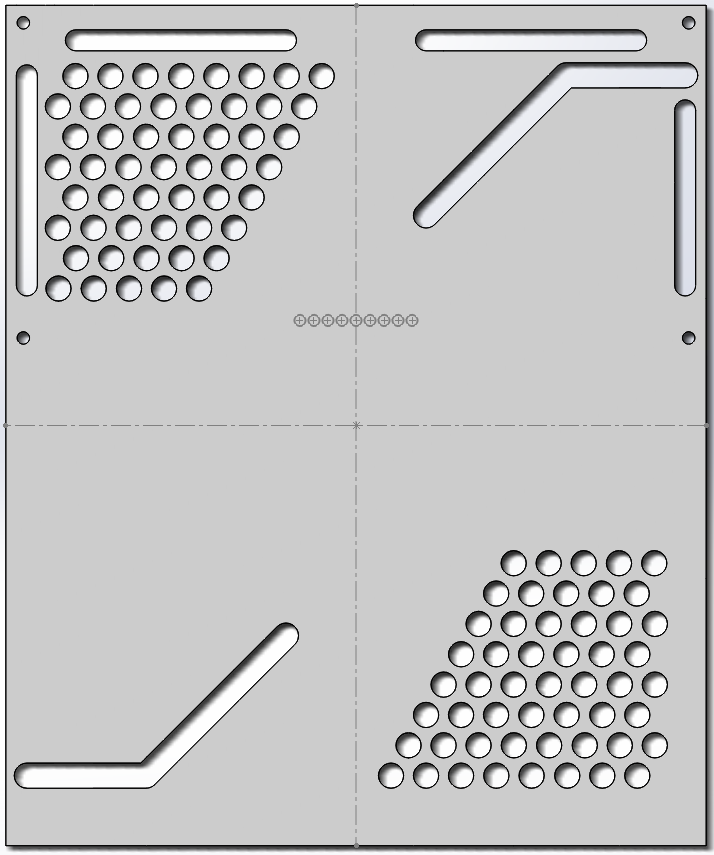
\includegraphics[width = \textwidth]{PR5Images/PlateALTopViewCAD.png}
				\caption{Top view of the aluminum plate.  Note the angled slot in the upper left and bottom right quadrants of the plate as discussed above.  The additional grid of holes was included to allow pedals with only two screws located on adjacent corners (such as the popular Ibanez TS-9) to be accommodated.  The additional vertical and horizontal slots allow the coaxial cables used to connect to the pedal's I/O to pass through the aluminum plate from the circuit board mounted underneath.  The four small holes are for mounting the circuit board.  The row of circles near the center of the piece show the locations of the electrodes used for the hot swapping connector.}
				\label{fig:Plate_AL_top}
			\end{subfigure}
			\begin{subfigure}{0.55\textwidth}
				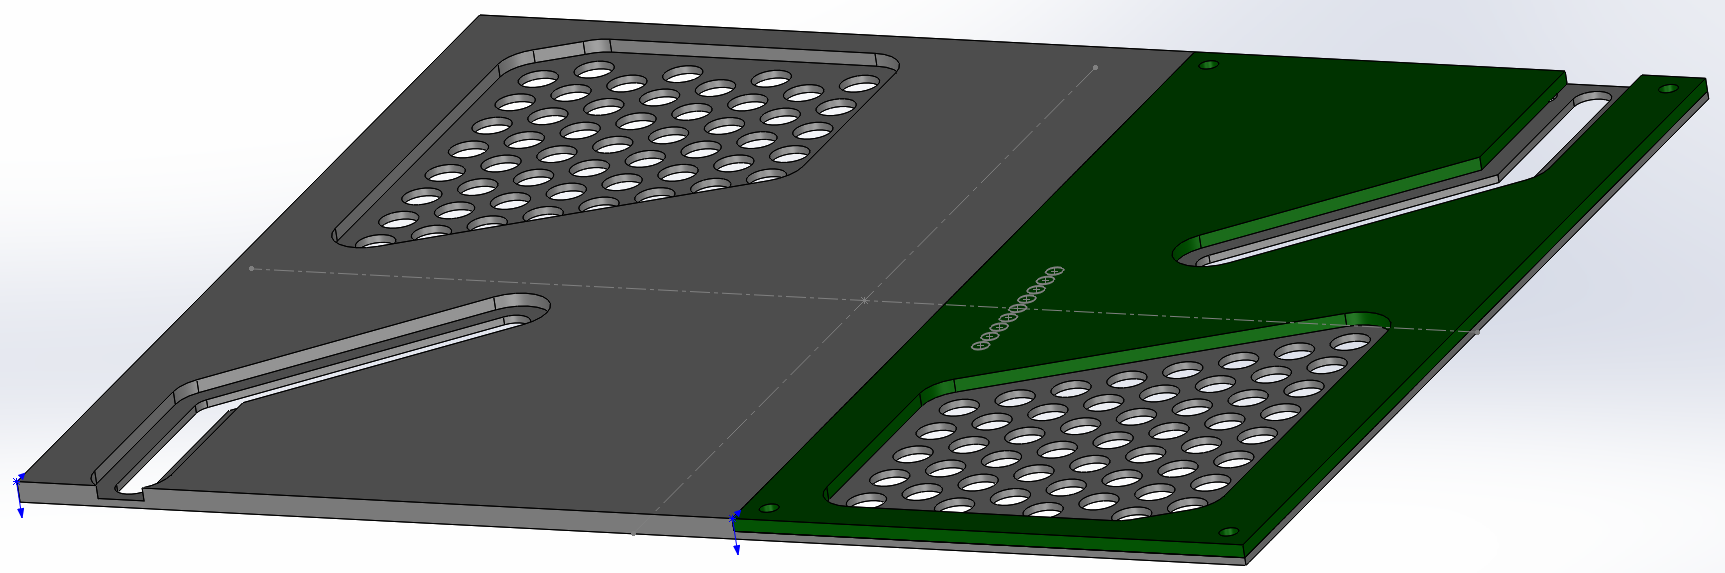
\includegraphics[width = \textwidth]{PR5Images/PlateAsmCAD.png}
				\caption{Assembly view of the plate, with the circuit board shown in green.  Note the pockets in the aluminum allowing the screw heads to catch without needed to waste the full 1/8" of thread length.  A pocket was also cut out for the circuit board to lie flush with the bottom surface.}
				\label{fig:NF_AP_sum}
			\end{subfigure}
			\caption{Universal adapter plate design.}
			\label{fig:finalplatedesign}
		\end{sidewaysfigure}

		The final design of the plate is shown in Figure \ref{fig:finalplatedesign}.  A 5" $\times$ 6" dimension was chosen to allow for room for the I/O connectors and larger pedals.


	\subsection{Hot Swapping Device}
			\subsubsection{Electrical Connection Mechanism}

		The core of this project is the hot swapping device.  The electrical connection that allows the transfer of power, audio, and control signals between the a universal adapter plate and the module containing the hot swapping device is vital.  Though a number of guitar pedals offer processing of stereo signals, most are fully monophonic, requiring only one input and output connection.  In addition, because almost every pedal uses a single supply (non-bipolar) voltage, the simplest scheme for connecting a plate to its receiver requires only four connections: Power, Ground, Input (Send), and Output (Return). This means that it is feasible to transfer the signal directly with individual physical connections, rather than some serial data protocol such as I$^2$S, which might be used if there were many inputs and outputs.  The use of ”hard-wire” connections also keeps the signal ”pure” by eliminating any unnecessary processing, which is an important consideration for marketing purposes.  

		Making a consistent electric connection between the plate and receiver calls for some sort of spring loaded connector.  They should be able to easily mate or break, but must maintain good contact when connected.  They should not require the two surfaces to be exactly aligned, and they should require only the single part to operate (instead of a matching male and female connector) for cost purposes.  Figure \ref{fig:springloaded} shows some examples of spring loaded connectors.  On the left are connectors typically used to connect boards together within a product. This class of spring connector is good for high pin count connections because of the large number of pins in a single unit, which are easy to manufacture cheaply. For example, the 00-9258 type connector from AVX Corp costs \$0.77 for 8 electrodes from Digikey. However, because these connectors are usually made for one time use when permanently assembling a product, they are not designed for repeated use. For instance, the 00-9258 part is has a lifespan of just 50 cycles according to its datasheet, which is certainly insufficient for this application. For an order of magnitude estimate, each plate needs to be able to withstand 100 cycles per day for at least 1000 days (though the cycles/day is likely lower and the total days is likely higher). This gives a ballpark estimate of 100,000 cycles minimum.  Spring loaded pins like those to the right in Figure \ref{fig:springloaded} were the preferred type of connector.  This type of connector, sometimes known as a ”Pogo Pin,” includes a spring loaded plunger that sheaths into a sleeve. These can be sourced through Digikey from Mill-Max, an industry standard manufacturer of milled connectors. They have excellent electrical and mechanical characteristics, including 20m\ohm contact resistance, minimum of 2 amp current rating, and a 1,000,000 cycle lifespan which makes them an excellent choice for this application.  The downside is in cost, as a single pin in the standard 0906 series costs \$0.44 each from Digikey, but the requirement for durability outweighs this drawback.

		\begin{figure}
			\centering
			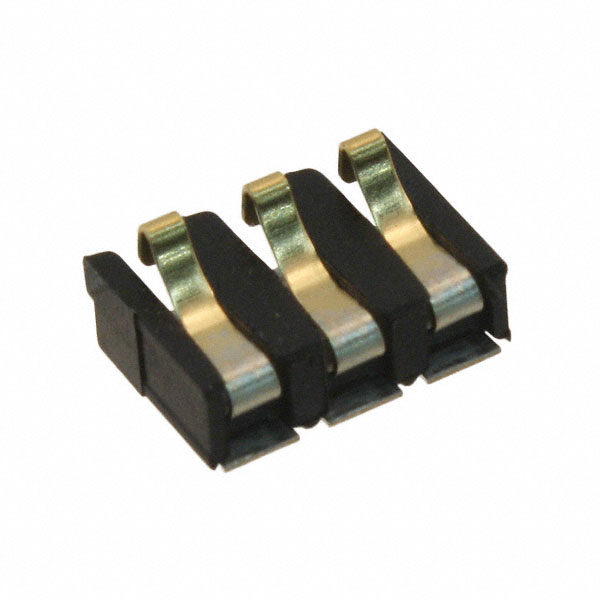
\includegraphics[width = 0.4\linewidth]{PR2Images/batteryconn}
			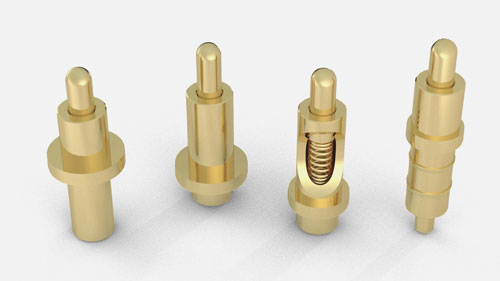
\includegraphics[width = 0.4\linewidth]{PR2Images/springpin.jpg}
			\caption{Examples of spring loaded connectors.  On the left is a battery type connector with leaf type springs.  On the right is a spring loaded pin type connector, often known as a "pogo pin".}
			\label{fig:springloaded}
		\end{figure}

		The 0906-1 model spring loaded pin was chosen because of its low cost relative to other series, and because it had a relatively short length (0.177") which reduces torques on the contact point between the pin and the circuit board due to any tangential force on the end of the pin, which is held in place only with solder.  This serves to increase durability; the through-hole mounting style was chosen over surface mount for the same reason.

		Initially, the design featured pogo pins of varying heights to enable a mate-first, break-last connection.  This was done with the intention of ensuring that the audio signals are never connected without the power also being connected, to avoid unnecessary pops and transients in the audio signal.  However, testing of a prototype hot swapping connector showed that the weight of the plate and pedal alone was not enough to activate both the taller and shorter pins, requiring additional force to make all connections.  Though this could have been fixed using a magnetic system to add the required force, a more sophisticated controlling mechanism (see below) was used to prevent the signal from being connected too soon, resulting in the same benefits as the varied height design without the issues with connection.

		Because most guitar effects pedals have only mono I/O and all of them support mono operation even if they do have stereo capability, the hot swapping device was designed to operate only in mono, although the design can easily be extended to stereo operation in the future.  This means that two pins are required for the audio signals, in addition to ground.  The power supply requires an additional power pin plus a second ground pin.

		\subsubsection{Pedal Power Selection}

		In order to maximize the compatibility metric, the solution should be able to supply the most commonly required voltage and current supplies.  Though 9VDC is the de facto standard voltage supply \cite{MyPedalData}, there are a number of effects that accept 12 or 18 VDC, which can allow their amplifiers to have a higher headroom.  There are some other less common power supplies, such as 24 VDC for some older Electro Harmonix products, or 9 VAC for pedals like the Line 6 DL4 \cite{Line6DL4manual}, but these are rarer, so the design focused on just the 9, 12, and 18 VDC supplies.  Users can select which power supply is used on each plate, and the desired power is automatically connected.

		In order to supply power to the plate, two schemes were considered.  The first was a parallel supply, where all three voltages are connected to the plate at once, and the user who sets up the plate for a particular pedal can choose which connector to attach the power connector to.  This would allow a single voltage regulator for each supply voltage to be used.  However, this could run into issues of current draw, where many pedals could potentially draw more current than the voltage regulator can handle.  In addition, this would mean long traces in the main board carrying this voltage, which might experience a voltage drop due to the resistance of these traces.  Figure \ref{fig:parallelpowerschematic} shows an implementation of such a scheme.

		\insertimage{0.5}{PR2Images/ParallelPowerSchematic.PNG}{Power supply implementation where all voltages are available at all times.}{fig:parallelpowerschematic}

		The other option was to use a single voltage regulator for each plate, with a controllable output.  This eliminates concern over voltage drops between different receivers, and allows each receiver to draw as much current as a single regulator can supply.  For more than two power outputs, this method saves pogo pins, as only two pins are needed to supply the power (in addition to ground), though it does require several pins to communicate which voltage is desired for the current plate.  Instead of multiple connectors to allow the user to select the power connection, this method would use some switch, such as a two position DIP switch, to allow the user to set a binary value which can be decoded on the receiving end into the proper signals needed to control the adjustable voltage regulator.  As the pogo pins are fairly expensive (about \$0.66 each), reducing the number of pins is a good way to save on cost.

		The LM317 is a canonical adjustable voltage regulator, with its level set via a voltage divider (see datasheet section 8.2 for a typical application and design requirements \cite{LM317datasheet}).  The LM317 takes an input voltage between 1.25 and 37 V, preferably with $V_I - V_O > $ 3 V.  The difference $V_{OUT} - V_{ADJUST}$ is then kept at 1.25 V with a feedback circuit.  As shown in Figure \ref{fig:LM317_typicalapp}, this 1.25 V reference and $R_1$ then set the current through variable resistor $R_2$ ($I_{Adj}$ is negligible) which controls the output.  The 240\ohm value for $R_1$ is a recommended value required to keep the output current high enough (over 3.5 mA) for a well regulated output.  The other diodes and capacitors are used to reduce ripple in the output.  Thus, $V_O$ can be given by

		\begin{align}
			V_O &= V_{REF}(1 + \frac{R_2}{R_1}) + I_{ADJ}R_2 \\
			&= 1.25 (1 + \frac{R_2}{240}) \quad \text{and} \\
			R_2 &= 240 \left( \frac{V_O}{1.25} - 1 \right) \\
			\label{eqn:LM317_R2}
		\end{align}

		However, a variable resistor for $R_2$ is not an easy method of setting the proper voltage for a user, because this would require individual tuning for each plate.  Instead, a set of switches is an easy mechanism for a user, who just needs to set the correct position of the switches.  A straightforward technique to use is switch in and out some additional resistors in parallel to a fixed $R_2$, as shown in Figure \ref{fig:adjustableregulatorschematic}.  Adding resistors in parallel reduces the effective resistance, reducing the output voltage, so the fixed $R_2$ should be calculated to set the maximum required output voltage, 18 VDC.  Using Equation \ref{eqn:LM317_R2} to calculate $R_2$ for an 18 V output gives $R_2 = 3.2 \text{\kohm}$. The current through $R_1$ and consequently $R_2$ is $i_{R_1} = 1.25/240 = 5.2$ mA.  

		\insertimage{0.8}{PR2Images/LM317_typicalapplication}{Typical Application of LM317, from datasheet.}{fig:LM317_typicalapp}

		\insertimage{0.8}{PR2Images/AdjustableRegulatorSchematic}{MOSFET controlled adjustable regulator, with 9, 12, and 18 VDC selectable output.}{fig:adjustableregulatorschematic}

		MOSFETs are a good choice for this switch application because of their relatively low on-resistance $R_{DSon}$.  The cheapest type of MOSFET available from Digikey was the NX7002AK type, a ubiquitous single N-channel device \cite{NX7002AKdatasheet}.  With a maximum $V_{DS}$ of 60 V, a maximum $I_D$ of 190 mA for $V_{GS} = 10$ V at $25^o$ C, and a typical $R_{DSon}$ of 3.7\ohm at $V_{GS}$ = 5V, this will work fine for this application, as would many standard MOSFETs.  In fact, because $R_{DSon}$ is on the order of Ohms while $R_2$ is on the order of \kohm, it can be neglected in the calculations for $R_3$ and $R_4$.

		For simplicity, assume the MOSFET gate signals will not be turned on together, and that Q3 is used for a 9 V output while Q4 is used for a 12 V output, as in the following truth table:

		\begin{center}
		\begin{tabular}{c c|c}
			Q3 & Q4 & Output Voltage (V) \\
			\hline
			0 & 0 & 18 \\
			0 & 1 & 12 \\
			1 & 0 & 9 \\
			1 & 1 & X
		\end{tabular}
		\end{center}

		Because the MOSFET's on resistance can be ignored, solving for the $R_3$ when $Q_3$ is turned on so $R_3$ and $R_2$ are connected in parallel to ground gives

		\begin{align}
			R_3 || R_2 &= R_1 \left( \frac{V_O}{1.25} - 1 \right) = 240 \left( \frac{9}{1.25} - 1 \right) = 1488 \\
			R_3 &= \frac{1}{\frac{1}{R_3 || R_2} - \frac{1}{R_2}} = \frac{1}{\frac{1}{1488} - \frac{1}{3200}} = 2.8 \text{\kohm}
		\end{align}

		Likewise, 

		\begin{align}
			R_4 || R_2 &= R_1 \left( \frac{V_O}{1.25} - 1 \right) = 240 \left( \frac{12}{1.25} - 1 \right) = 2064 \\
			R_4 &= \frac{1}{\frac{1}{R_4 || R_2} - \frac{1}{R_2}} = \frac{1}{\frac{1}{2064} - \frac{1}{3200}} = 5.8 \text{\kohm}
		\end{align}

		Compute the power dissipated across these resistors to determine their necessary ratings.

		\begin{center}
		\begin{tabular}{c c|c}
			R (\kohm) & V (V) & P (mW) \\
			\hline
			$R_1$ = 0.240 & 1.25 & 6.51 \\
			$R_2$ = 3.2 & 18 - 1.25 = 16.75 & 87.68 \\
			$R_3$ = 2.8 & 12 - 1.25 = 10.75 & 41.27 \\
			$R_4$ = 5.8 & 9 - 1.25 = 7.75 & 10.36
		\end{tabular}
		\end{center}

		Even with a 10\% safety margin, these resistors can all be 1/10 watt.

		\subsubsection{Hot Swap Event Detection}

		To perform the automatic bypassing feature, the receiving side of the hot swapping connector must detect whether or not a plate has been inserted. To do this, some of the same type of electrodes used to make connection between the plate and the receiver for signal and power where used as SPST switches.  When no plate is inserted, the switch is open, and when a plate is inserted, the switch closes. This can signal some logic circuitry to actuate the actual signal switching device.  To reduce transients that could result from suddenly connecting a plate and allowing the signal to flow before all of the necessary connections (Power, Ground, Input, and Output) are made, the receiver should wait to switch the relay from bypass to active until all of the pins have made their connections.

		Two of these switch pins were used.  Out of convenience and the ability to integrate Mill-Max's complementary pogo pin targets if necessary, the whole set of pins were arranged in a single row with 0.1" pitch.  The switch pins were placed on either end of this row.  Assuming a flat plate, this means that if both of the switch pins have made contact with the plate, then the rest of the pins must have also made contact.

		Electrically, these switch pins were each connected to an input of a microcontroller, with pull up resistors enabled.  When no plate is present, these GPIO are pulled high through these pull-ups.  On board the plates, the mating electrodes for the switch pins are both connected to the ground electrode, so when a plate is inserted into the hot swapping receiver, the switch pins are connected to ground and the microcontroller inputs are pulled down.  A logical AND on the debounced values of these switched is used by the microcontroller to determine if the plate has been inserted.

		The debounce routine used for these pins is performed in parallel on each of them.  It ensures that the value of the GPIO has remained constant for $20ms$ after it detects a change in the pin before the signal is asserted to the rest of the program.  The debouncing of the switch pins also allows the power and audio signal pins to connect before the audio signal is sent to the pedal.

		\subsubsection{Hot Swap Event Actuation}

		Once the microcontroller detects that a plate has been inserted or removed from the hot swapping receiver, it must initiate the actual signal switching.  The primary function of the hot swapping device is to automatically bypass any receivers that do not currently have a plate inserted, so the choice of switching element is a key part of the design. The basic choice here was between solid state analog switches or electromechanical relays. The major design considerations for this choice are the signal to noise ratio, and the frequency response of the switching element. 

		The initial value measured for the noise floor for an electric guitar was near $-90dBV$.  Guitar pickups convert the mechanical energy of the vibrating strings to electrical energy via a coil of wire. When the string vibrates in the magnetic field of a permanent magnet situated underneath, current is induced in the coil. In an ideal environment, there should be little source of self noise because of the passive simplicity of this device, so any noise in the guitar signal is a result of the environment. As such, the signal to noise ratio of a guitar can vary significantly based on the guitar’s environment. For example, guitar pickups are well known for their susceptibility to 60Hz line noise. Therefore, the measured 90dBV signal to noise ratio should be taken as a minimum value, with 100dBV or more preferable. While solid state switches are more size, cost, and power efficient than mechanical relays, they may not have adequate signal to noise specifications, as well as crosstalk between channels on the same chip. For example, the MT8808 Analog Switch Array lists no specification on the device’s signal to noise ratio, though it does boast a reasonable $-90dB$ crosstalk between any channels for a 10kHz input with a 600\ohm load. The feed-through when a channel is off is listed as $-95dB$ though, which is does not far exceed the minimum measured value for guitar signal to noise ratio, which could be an issue. On the other hand, relay bypassing utilizing mechanical switches has no issues with signal to noise ratio, which would make it suitable for use in this project.

		As a minimum, the system should accommodate signals across the full range of human hearing, which is typically noted as 20Hz - 20kHz. While this is the minimum acceptable range, there should also be allowance for lower and higher frequencies, which when used as input to a distortion effect can create inter-modulation distortion with frequencies in the audio range. Neither of these ranges will be an issue however. In the case that switching is accomplished with a solid state device, these are designed for frequency responses up to the tens of MHz range (the MT8808 has a 3dB frequency response of 45MHz), which is far greater than required. If mechanical relays are used, there will likewise be no issues with frequency response in the audio range.

		\insertimage{0.4}{PR2Images/GuitarPickupModel}{Model of guitar circuit.  These values are highly dependent on the particular pickups.  The potentiometer is either 250\kohm or 500\kohm.}{fig:guitarpickupmodel}

		These considerations suggest a preference for using mechanical relays despite their costs. An additional reason is some of the interactions between the circuits on the guitar and in the first engaged pedal. As mentioned above, the guitar pickup is made from a coil of wire, typically about 42 AWG with thousands of turns around a 6 inch or so circumference bobbin. This long thin wire produces a DC resistance on the order of 10\kohm, which itself is quite a high output impedance, and the inductance and some parasitic capacitances from within the pickup will result in a frequency dependent output impedance with the potential to interact with a connected circuit block with sufficiently low input impedance. In addition, the position of the guitar’s volume potentiometer can affect the output impedance (see Figure \ref{fig:guitarpickupmodel} for a model of a guitar pickup and volume control circuit). There are a number of guitar pedals known for their interaction with the guitar’s volume knob.  This does not follow the rule of thumb suggesting the input impedance should be an order of magnitude greater than the output impedance of the previous circuit stage, which means that there will be interactions between the guitar and this pedal.

		Whether or not these interactions are good or bad, they have an undeniable effect on the sound and feel of playing the guitar through this pedal. Inserting a buffer, including a solid state switch, between these circuit elements would destroy this interaction, and thus would prevent the solution from being an effect tool for comparing different pedals. Therefore, the signal path should pass through no buffers when all receivers are bypassed, and electromechanical relays should be used to perform the switching.

		To choose the relay, several criteria were considered, as listed in Table \ref{tab:relay_criteria}.  During the prototype design, the Kemet EA2-5SNJ was chosen as the best candidate.  The single coil latching Form-C DPDT relay had the best combination of the desired properties for the best price.  However, when it came time to build the full system with multiple modules in the spring, the EA2-5SNJ had become obsolete, and had to be replaced with the similar UD2-5SNU.

		\begin{table}
		\begin{center}
		\begin{tabular}{ |c p{3in} c| }
		\hline
		\multicolumn{3}{|c|}{\large Relay Selection Considerations \normalsize} \\
		\hline
		Criteria & Description & Desired Value\\ 
		 \hline
		Coil Voltage 	& The voltage required to activate the relay.  Higher voltages typically require less current because of higher coil resistances.  While it is beneficial to minimize relay coil current, it is often easier to use a lower coil voltage for easier interfacing with logic circuits or microcontrollers.  & 5V \\
		Switch Type 	& DPDT, SPDT, SPST, etc... a DPDT allows a single device to activate the bypassing for an entire hot swapping device.  & DPDT \\
		Actuation Type 	& Non-latching, Single Coil Latching, Double Coil Latching.  Non-latching is simplest but requires continuous current to keep relay in "set" state.  Both latching types require more complex control circuits & Latching \\
		Contact Type 	& Form A, B, C.  The first two relate only to SPST.  Form C indicates that a xPDT relay will break one connection before making the other, which is desired so two outputs are never connected together simultaneously. & Form C  \\
		Cost 			& This is self explanatory, but it is important to consider the total cost required to perform the desired action.  For instance, two SPDT relays would be required to do the same job as a single DPDT, so the SPDT relays would need to each be less than half the price of the DPDT to be preferred. & Minimum per pole \\
	   	\hline
		\end{tabular}
		\caption{Considerations used to select particular relay device.}
		\label{tab:relay_criteria}
		\end{center}
		\end{table}

		These relays use a single-coil latching actuation method, where the coil is s energized in one polarity to set the switch to one position, and is energized in the opposite polarity to set the switch to the other position. This calls for an H-bridge style driver.

		\insertimage{0.6}{PR2Images/DiscreteHBridge.png}{Discrete H Bridge implementation.  The inductor coil K1C load is the relay coil.}{fig:DiscreteHBridge}

		A standard discrete H bridge like the one shown in Figure \ref{fig:DiscreteHBridge} uses a quartet of transistors to power a load in either polarity or not at all.  When the two transistors in opposite corners (such as Q1 and Q4) are turned on at the same time, current flows through these transistors and the load, in this case the latching relay coil.  When it is time to set the relay's switch to the opposite position, the other two transistors are turned on instead and the load is energized with opposite polarity.  This implementation features garden-variety 3904/3906 type BJTs, which can supply plenty of current for the relay coil (just $5V/250\Omega = 20 mA$), though these many other transistors would work.  D1-D4 are flyback diodes for the inductive relay coil.  To provide a load current of 

		\begin{align}
			i_{load} &= \frac{5V - V_{CE_4} - V_{CE_1}}{250 \Omega} = 18.4 mA
		\end{align}

		the base current of the transistors is related to the collector current by

		\begin{align}
			I_B &= \frac{I_C}{\beta}
		\end{align}

		The 2N3904 has a $\beta$ between 100 and 300 for a 10 mA $I_C$, so assuming $\beta = 200$ gives a required base current of

		\begin{align}
			I_B &= \frac{18.4mA}{200} = 92 \mu A \quad \text{and} \\
			R_2 &= 4.3V/92\mu A = 43 k\Omega
		\end{align}

		For a 10\% tolerance, use a $39k\Omega$ to ensure the transistor is turned fully on.

		A major issue with the H-bridge design is that both sets of transistors can never be turned on at the same time.  This would create a low impedance path from power to ground, cause high currents and potential damage to the circuit.  Though more of an issue in PWM motor control, a common application of the H-bridge, this "shoot-through" can occur when one set of transistors is switched on just as the other set is switched off.  Special protection must be taken to prevent such issues.

		For this reason, dedicated H-bridge driver ICs are offered.  One canonical example is the L298 dual H-bridge driver \cite{L298datasheet}.  It includes protection logic to prevent shoot-through and has enable inputs for each bridge.  This would be a good choice of driver, but for the price, which is about \$5 per chip from Digikey, which is more than the cost of the two relays it would be driving.  This is especially striking when considering that the cost of the MMBT3904 and MMBT3906 are \$0.10 and \$0.13 each.  For an integrated solution to be viable, it should not cost more than the relays it is driving.  Other options are the LV8548MC-AH \cite{LV8548MCdatasheet} and the LB1948MC \cite{LB1948MCdatasheet} from ON Semi.  These also have logic to prevent shoot through, and a thermal shutdown function to protect the chip.  Better yet, the LV8548MC-AH is available in a 10-SOIC package for \$1.33 each, putting the per-relay cost at just \$0.67.  This is on par with the cost of four of discrete transistors mentioned above.  Because the additional circuit protection justifies the use of this driver.

		Operation of the relay requires some logic to convert the plate detect signal to the proper signals required to switch the relay.  Although the EA2-5SNJ has a maximum operate time of 3 ms when driven at 100 mW (which is the nominal power applied to this 5V relay), the relay expects a pulse of more than 10 ms in duration \cite{EA2datasheet}.  As these should only be sent on the appropriate transition of the plate detect signal, an edge detector combined with a pulse generator should be used as the control logic, as shown in Figure \ref{fig:HBridgeCTRL_Block}.

		\insertimage{0.95}{PR2Images/HBridgeCTRL_Block.PNG}{Block Diagram depicting the processing of the plate detect signal needed to drive the H bridge and ultimately switch the relay.}{fig:HBridgeCTRL_Block}

		Although discrete logic implementations were explored, a microcontroller was the better option because of its re-programmability and the need for a number of logical operations throughout the design.  An Atmel AVR ATTiny40 was chosen for the prototype design for its low cost yet adequate GPIO count.  However, its lack of on-chip debugging proved to be an inconvenience during prototype fabrication and testing, and it proved to be inadequate in terms of GPIO count when the time came to design the full module.  Therefore, the final module design used an ATMega3209 to stay in the same design environment but reap the benefits of a more fully featured microcontroller.

		The function of the circuits described above were implemented in code on the chosen microcontroller.  A block diagram of all the necessary functions for a single receiveri s shown in Figure \ref{fig:MicroBlockDiagram}.

		\insertimage{0.95}{PR2Images/ReceiverBlockDiagramMCU.PNG}{Hot swapping receiver block diagram.  The blocks within the shaded region corresponding to the microcontroller were implemented in firmware.}{fig:MicroBlockDiagram}

	\subsection{Analog Signal Routing}
	

	In order to allow the user to set up complex signal routing configurations, an analog signal routing matrix needed to be designed.  To keep the modules simple and independent while still providing a large variety of routing options, each module is equipped with a 2x2 mixer.  These options become available when the modules are connected together as in Figure \ref{fig:system_block}.

	\subsubsection{Routing Architecture}

	Each module contains a two input, two output mixer. Each of the two outputs 1 and 2 can be connected to either input $A$ or $B$, as well as the sum of the two inputs $A + B$.  Table \ref{tab:routing_outputs} shows the possible outputs.  As can be seen, there are only three signals that must be available for the output.

	\begin{table}
	\begin{center}
	\begin{tabular}{ |c|c c| }
	\hline
	 Permutation & Output 1 & Output 2 \\ 
	 \hline
	 1 	& $A$ 	& $A$ \\  
	 2 	& $A$ 	& $B$ \\
	 3	& $A$ 	& $A+B$ \\
	 4	& $B$ 	& $A$ \\
	 5	& $B$ 	& $B$ \\
	 6	& $B$ 	& $A+B$ \\
	 7	& $A+B$ & $A$ \\
	 8	& $A+B$ & $B$ \\
	 9	& $A+B$ & $A+B$ \\
	 \hline
	\end{tabular}
	\caption{List of the $2^3$ possible output signals for each routing module.}
	\label{tab:routing_outputs}
	\end{center}
	\end{table}

	The routing mechanism was designed with this in mind.  For the same reasons that relays were chosen to actuate the signal switching in the hot swapping receiver subsystem, they are also used here.  This is essential especially when an output is connected directly to an input, such as permutation 2 in Table \ref{tab:routing_outputs}, which will preserve both the SNR and frequency content of the signals in addition to the signal's output impedance.  However, when a summed output is chosen ($A+B$), the signals must necessarily pass through a summing amplifier, which will result in a low impedance output anyways.  In this instance, the use of a mechanical relay is not strictly necessary.

	The specific implementation of the routing subsystem is shown in Figure \ref{fig:routingschem}.  Each output selector is in essence a three-to-one analog multiplexer.  The requirement for mechanical relays when the sum output is not selected requires the use of mechanical relays throughout, as each can only switch between two inputs.  Thus, each three-to-one multiplexer includes two of the same DPDT relays used for the receivers, despite not all of the throws being in use, as they were cheaper than any SPDT relay.  Using the same UD2-5SNU relays also minimizes additional components on the BOM.  The use of latching relays here is even more beneficial than in the receiver, as these relays will likely be set in a position for long periods of time, so the reduced current and heat dissipation compared to a non-latching relay is very beneficial.

	To generate the summed $A+B$ signal, a standard inverted summing amplifier is used.  The resistors were chosen to each be $10K\Omega$ so that each input is at unity gain.  Higher resistor values were avoided to reduce thermal noise.  However, the input impedance to the inverted amplifier is just the value of the input resistor, so non-inverting op-amp buffers are required to prevent preceding circuits on $A$ and $B$ from interacting with the summing amplifier, which in this case is undesirable.  As this already requires three op-amps and the output signal would be inverted, an additional unity gain inverted buffer is used at the output to re-invert the signal, resulting in $A+B$.

	The $A$ and $B$ inputs are each connected through a decoupling capacitor to their respective op-amp buffer inputs, and are pulled to the reference voltage via 1M resistors.  The 1M resistors were chosen to prevent the $A$ and $B$ signals from being heavily loaded down, especially when the signal passes a number of these between the input and output.  When the signal sees several of these in parallel, the equivalent resistance decreases quickly, which can result in issues, so a larger biasing resistance is desirable.  A large resistor value here also means the capacitance of the decoupling capacitor can be less to maintain a similar cutoff frequency, and it will be cheaper to have a higher quality plastic film or C0G ceramic capacitor in a smaller value.  The limit to choosing a very large resistor is the thermal noise, which may become a concern even with this value.  If this becomes an issue, the values can be adjusted once the board has been fabricated.  The cutoff frequency for the high pass filter formed by pull-up resistor and the decoupling capacitor should have its cutoff frequency on the order of 5-10Hz so it will pass the full audio range.  For a 1\Mohm resistor, this means

	$$ C = \frac{1}{2\pi R F_c} = \frac{1}{2\pi (1 \text{\Mohm}) (10 \text{Hz})} = 15.8 \text{nF}$$

	Because this is on the high end of the frequency range, the next larger standard value capacitor, 0.022\uF, is used.  Kemet offers a 0.022\uF film capacitor in through hole mounting for just \$0.25.  The film capacitors are more linear and have lower ESR and self inductance than typical ceramic caps, making them suitable for audio signal path usage.  The resistors can be standard.

	The op-amp selected should have low noise, low input bias current to prevent loading the input signal lines, and a rail-to-rail output to maximize headroom.  For op-amps compatible with a supply of 24V or more, Texas Instrument's OPA1679IDR is a good candidate.  At \$1.20 from Digikey, it is not cheap, but its datasheet claims 0.0001\% THD+N, a 10 pA max input bias current, and voltage output within 800mV of each rail \cite{OPA1679IDRdatasheet}.  These specs compare admirably to the TLV4172IDR and OPA4172IDR, each of which are twice the price.  Because there are not too many components in the audio path and its value as a reliable reference is paramount, it is appropriate to use more expensive and higher quality parts here.  The schematic for the analog signal routing subsystem is shown in Figure \ref{fig:routingschem}.  

	\begin{sidewaysfigure}
		\centering
		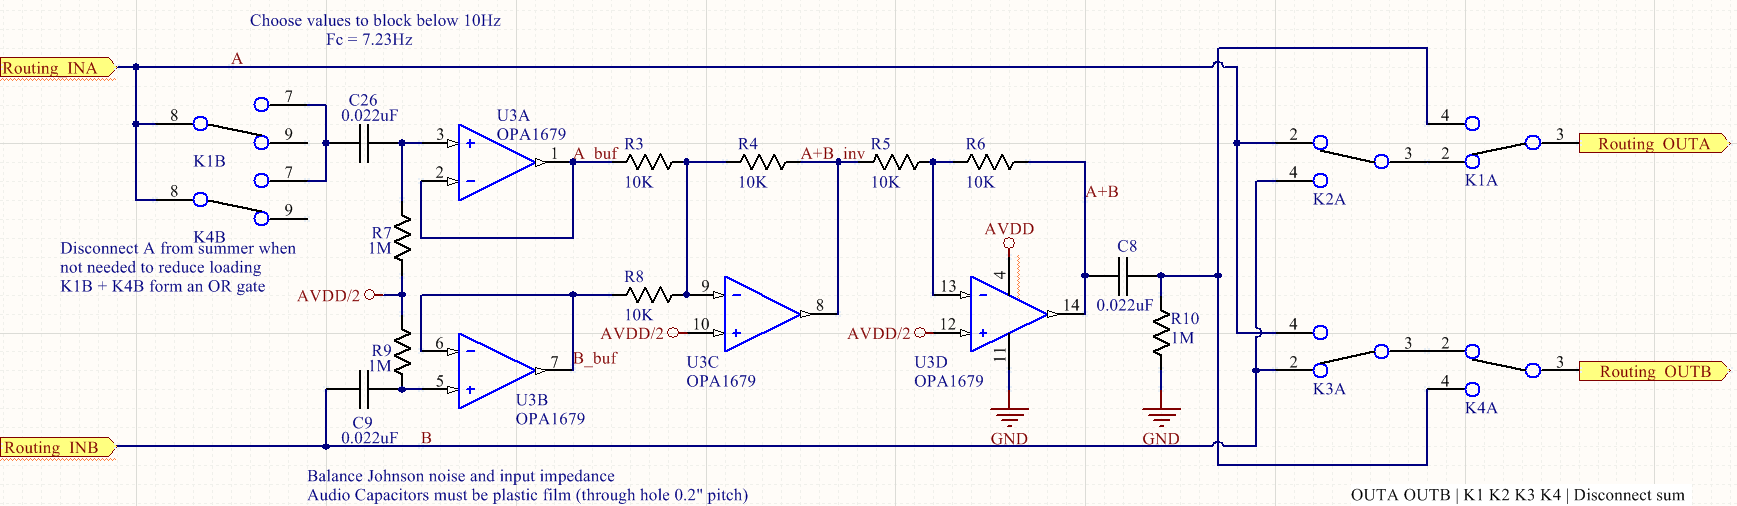
\includegraphics[width = \textwidth]{PR4Images/RoutingSchem.PNG}
		\caption{Schematic of analog signal routing subsystem.  Note that the second halves of two out of the four routing relays are in use.  The relays associated with choosing between a summed output or not are used to create an OR gate which will disconnect the biasing resistors from the $A$ signal, reducing the loading whenever the summer is not needed.}
		\label{fig:routingschem}
	\end{sidewaysfigure}

	\subsubsection{Analog Voltage Supply}

	
	This summing amplifier and related circuitry requires its own analog supply voltage.  In the worst case, the maximum voltage swing of each input signal $A$ and $B$ should be no more than 18Vpp, which is the maximum supply voltage available to a pedal from a receiver.  This means that the summing amplifier should ideally be able to swing 36Vpp.  However, the power supply currently being used provides 24VDC.  This means that without modification, the summing amplifier will not be able to sum all possible signals without clipping.

	There are several possible solutions to this issue.  One would be to change the device's power supply.  Moving to a chassis mount 48V supply like Mean Well's LRS-150-48 \cite{datasheet:LRS-150-48} (\$22.50 from Digikey \cite{digikey}) would allow for plenty of headroom and could provide much more current (in this case 3.3A), enough for six pedals each drawing 500 mA while leaving some budget for the device's own circuits.  A new power supply could be chosen to avoid the issue of switching noise in the audio range; the switching frequency of the LRS-150-48 is 65kHz, well above the audio spectrum.  Linear regulators could be used to drop the input voltage to the desired level, in this case just above 36V.  This supply could then be split with a resistive divider to provide the virtual ground needed for the op amp summer.  Brick-type supplies in this voltage and current range are prohibitively expensive, such as the PSA120U-480L6 from Philhong USA for \$38 \cite{digikey}.

	A second option would be designing an on-board boost-buck converter to create the desired supply voltages.  In this case, this switching supply could be used to generate an arbitrary voltage, so a bipolar 18V or 24V set of rails could be created.  This would allow for sufficient headroom for the summing amplifier, and by virtue of the bipolar supply would not require AC coupling the summed signals to a virtual ground: they could remain DC coupled.  A switching supply would also be more efficient than a linear regulator.  However, the added complexity of implementing a switching voltage regulator, is probably not worth the benefits.  Noise from the on-board supply would need to be carefully controlled so as to avoid corrupting the audio signals.  In addition, a linear regulator would likely still be used to really clean up the residual ripple from a switching regulator.

	The third option is simply using a linear regulator to even out the current 24V supply and allowing the summing amplifier to clip at a lower voltage.  This is not as big an issue as it seems at first.  Though the worst case scenario is two 18Vpp signals being summed in phase, this would require the user to be using two pedals in 18V mode at full output level.  The more likely use case with two 9V pedals would work fine with the 24V supply.  If the user does cause the summing amplifier to clip, they can simply reduce the output level of the two pedals.  In addition, if the amplifier were able to sum two outputs to 36Vpp, this would cause the next pedal in the chain to clip as well because of its voltage could be 18V at maximum, so the 36Vpp output would only be usable at the input of the amplifier where it would not clip the amplifier input.  This is also the simplest option, as it requires only a linear regulator to clean up the 24V input and a resistive divider to generate the virtual ground reference voltage.  

	\begin{table}
	\begin{center}
	\begin{tabular}{|c|p{2in} p{2in}|}
	\hline
	Option & Pros & Cons \\
	\hline
	Change Power Supply 	& Allow increased headroom for summing amplifier.  Increase current capacity for entire system.  Possible to fix switching noise issue. 
								& Potentially expensive for quality supply with the required high current and voltage.  No guarantee that all issues will be solved. \\
	On-board Switcher 		& Bipolar supply possible for DC coupling.  Arbitrary headroom for this application.  More efficient than linear regulators. 	
								& Complicated.  Potential for its own noise issues would require mitigation. \\
	No Action 				& Easy.  Cheap.  Still satisfies most operating conditions. Low Noise.
								& Limited headroom.  Inefficient. \\
	\hline
	\end{tabular}
	\caption{Summary of analog supply voltage regulation options.}
	\label{tab:pwrsupplyproscons}
	\end{center}
	\end{table}

	Because of the simplicity of the third option and its relatively limited negative effects, this method was chosen to provide the supply for the summing amplifier.  To maximize the dynamic range of the summing amplifier, the regulated supply rail should be as close as possible to the 24V input.  The 200mV noise spec on the power supply means that the regulator must drop at least 200mV.  An adjustable regulator would be useful here to precisely set the output voltage.  The LM317 adjustable regulator used for the receiver is one option.  However, it's minimum 3V drop between input and output means that the analog supply rail cannot be set any higher than 21V \cite{LM317datasheet}.  This decreased headroom is not desirable, so a lower dropout device would be preferable.  The LM2931C is an adjustable low dropout voltage regulator which can be set output anywhere from 3 to 24V with a maximum dropout voltage of just 0.6V, about one diode drop.  This means that the analog supply voltage AVDD can be set very close to the 24V input.

	The LM2931C's datasheet provides design guidelines for setting the output voltage, but it follows the same principle as the LM317 divider used for the receiver.  The datasheet gives the following equation to set the output \cite{LM2931datasheet}:

	$$ V_{out} = V_{ref} \left( 1 + \frac{R_2}{R_1} \right) + I_{adj}R_2 $$

	which also accounts for the small current on the ADJ pin.  The datasheet also suggests keeping

	$$ 22.5\text{\kohm} \ge \frac{R_1R2}{R_1 + R_2} $$

	According to the electrical characteristics page, the reference voltage $V_{ref} = 1.2V$, and the adjust pin current $I_{adj} = 0.2\mu$A.  Setting $R_1 = 27$\kohm and $R_2 = 487$\kohm gives an output voltage of 23V, which is ideal.  The 487\kohm resistor is not one of the standard values, but slight adjustments in resistance to get to a nearby value cause too much of a change in voltage.  The output must also have a capacitive load on the order of 10\uF for stability.  Figure \ref{fig:AVDDreg} shows the circuit implementation of the regulator.

	\begin{figure}
		\centering
		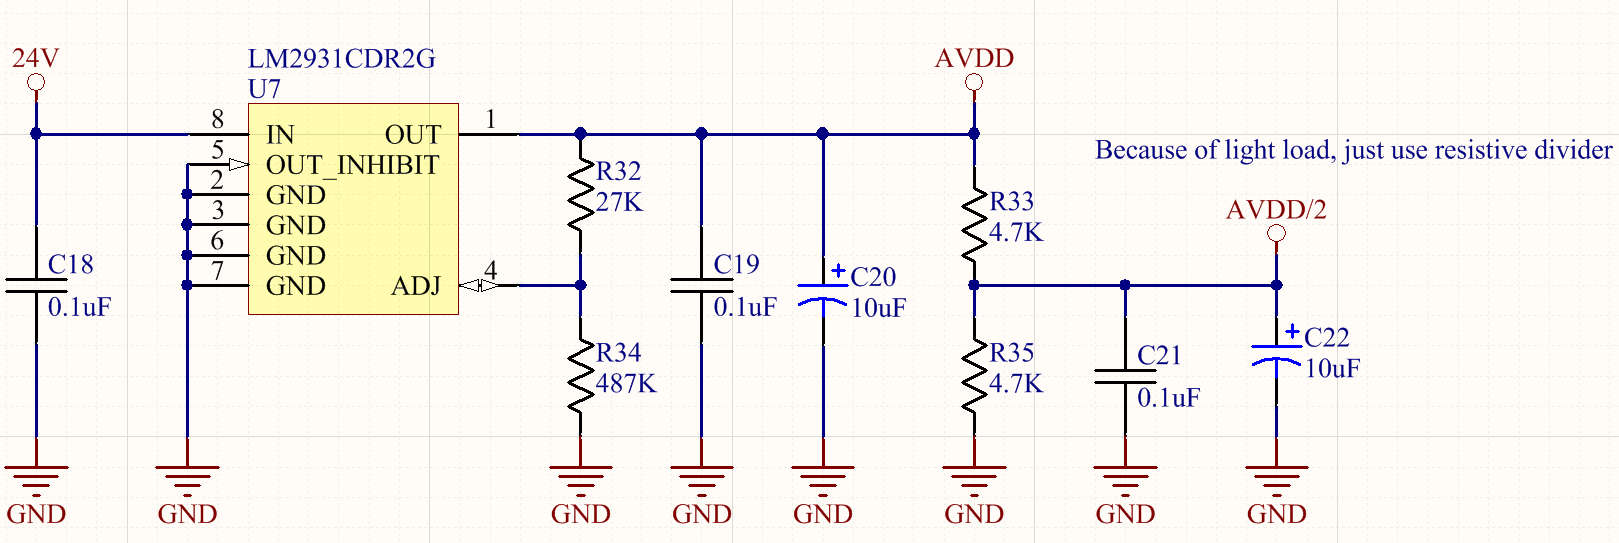
\includegraphics[width = \textwidth]{PR4Images/AVDDregulator.PNG}
		\caption{AVDD regulator design using LM2931C low voltage adjustable regulator and a resistive divider to provide a large split supply.}
		\label{fig:AVDDreg}
	\end{figure}

	From this analog supply voltage, a virtual ground can be produced from a simple resistive divider circuit.  Though in theory this is susceptible to sagging due to large current loads, this should not be an issue for this application because the reference voltage is connected only to the inputs of two op-amps, and tied to the audio signal through large resistors.


	\subsection{Signal Routing User Interface}
		
	The above analog signal routing subsystem must be controlled by the user.  Because this device is designed to simplify the user experience, the user interface should be intuitive to use; no or few instructions should be needed to operate it.  The user interface should clearly indicate the current state of the signal routing, and the method by which the user can change the routing should be likewise linked to the physical signal connections being made.  To avoid disrupting the user from their focus on audio, the interface should be primarily visual and tactile in nature, as opposed to auditory.  For these reasons, the indication and actuation elements should be meshed, taking the form of push buttons with an integrated light.

	As described in Table \ref{tab:routing_outputs} above, each of the two inputs can be connected to each of the two outputs.  This includes cases where both inputs are connected to one or both of the outputs.  In no scenario can an output be connected to no input, which means that the user will never experience any "dead spots" where no sound can be heard.

	Qualitative tests were used to determine the effectiveness of such an indicator light.  An 8" $\times$ 1/2" $\times$ 1/4" clear acrylic sheet was cut using a laser cutter.  One side of this sheet was engraved with the same laser cutter in a continuous pattern to provide a rough surface off which light can reflect and refract.  An LED was lit and place on one end of the sheet, facing the 1/2" $\times$ 1/4" rectangular side.  When the LED was held within 5mm or so of the face, the acrylic appeared to illuminate when viewing either of the 8" $\times$ 1/2" faces.  Though a white LED was originally planned, a blue color shows more contrast with the surrounding environment, so this is the color that will be used.  This rapid prototyping was conducted in a brightly lit machine shop, with lighting conditions similar to that expected in a guitar retail store, suggesting that this system will work in its intended environment.

	\begin{figure}
		\centering
		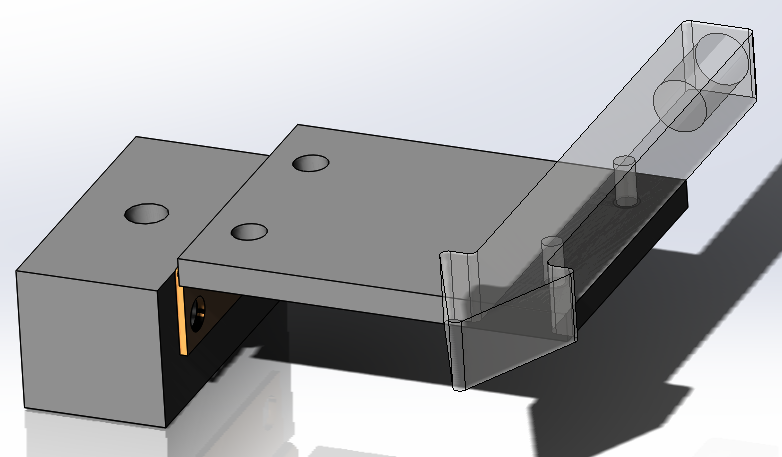
\includegraphics[width = 0.8\textwidth]{PR5Images/UIArrowCloseupCAD.png}
		\caption{Individual button setup for user interface showing the lever arm used to hold the indicator arrow light.}
		\label{fig:UIButtonCloseUp}
	\end{figure}

	Figure \ref{fig:UIButtonCloseUp} shows a single assembly for a light-button of this type, in this case illustrated without the button (the button and the lighting assembly are in separate CAD assemblies).  The clear arrow on top is a piece of 1/4" acrylic, with the bottom side raster textured on a laser cutter.  When light is injected into the acrylic from the side, it reflects off of this textured surface, which allows the light to be visible when looking down from the top view angle.  This arrow is mounted on a lever attached to a hinge, which is visible in a brass color.  This hinge pivots on a mounting block which is used to set the height of the arrow button.  A small pushbutton of the EVQ-22705R \cite{EVQ-22705Rdatasheet} variety is mounted underneath the lever directly below the center of the arrow.  When a user wants to select a routing connection, they would press down on the arrow.  This force produces a torque which allows the hinge to rotate down slightly, engaging the push button which pulls down an input on the microcontroller.

	Although this diagram illustrates a slot for a through hole LED to be inserted into the acrylic itself, rapid prototype testing indicated that the drill process for producing this slot causes too much texturing to the surface which interrupts the regular propagation of light the acrylic.  Therefore, small surface mount LEDs were used instead with no need for drilling.  

	\subsubsection{Button Layout}

	The exact layout of the buttons should be physically intuitive for the user to select the active inputs for each output.  The physically layout of the receivers is on a $3 \times 2$ grid.  The signal routing subsystems are used to connect the paired receivers on adjacent columns.  Figure \ref{fig:OverallUILayout} shows the overall layout of the receivers and the buttons.

	\begin{figure}
		\centering
		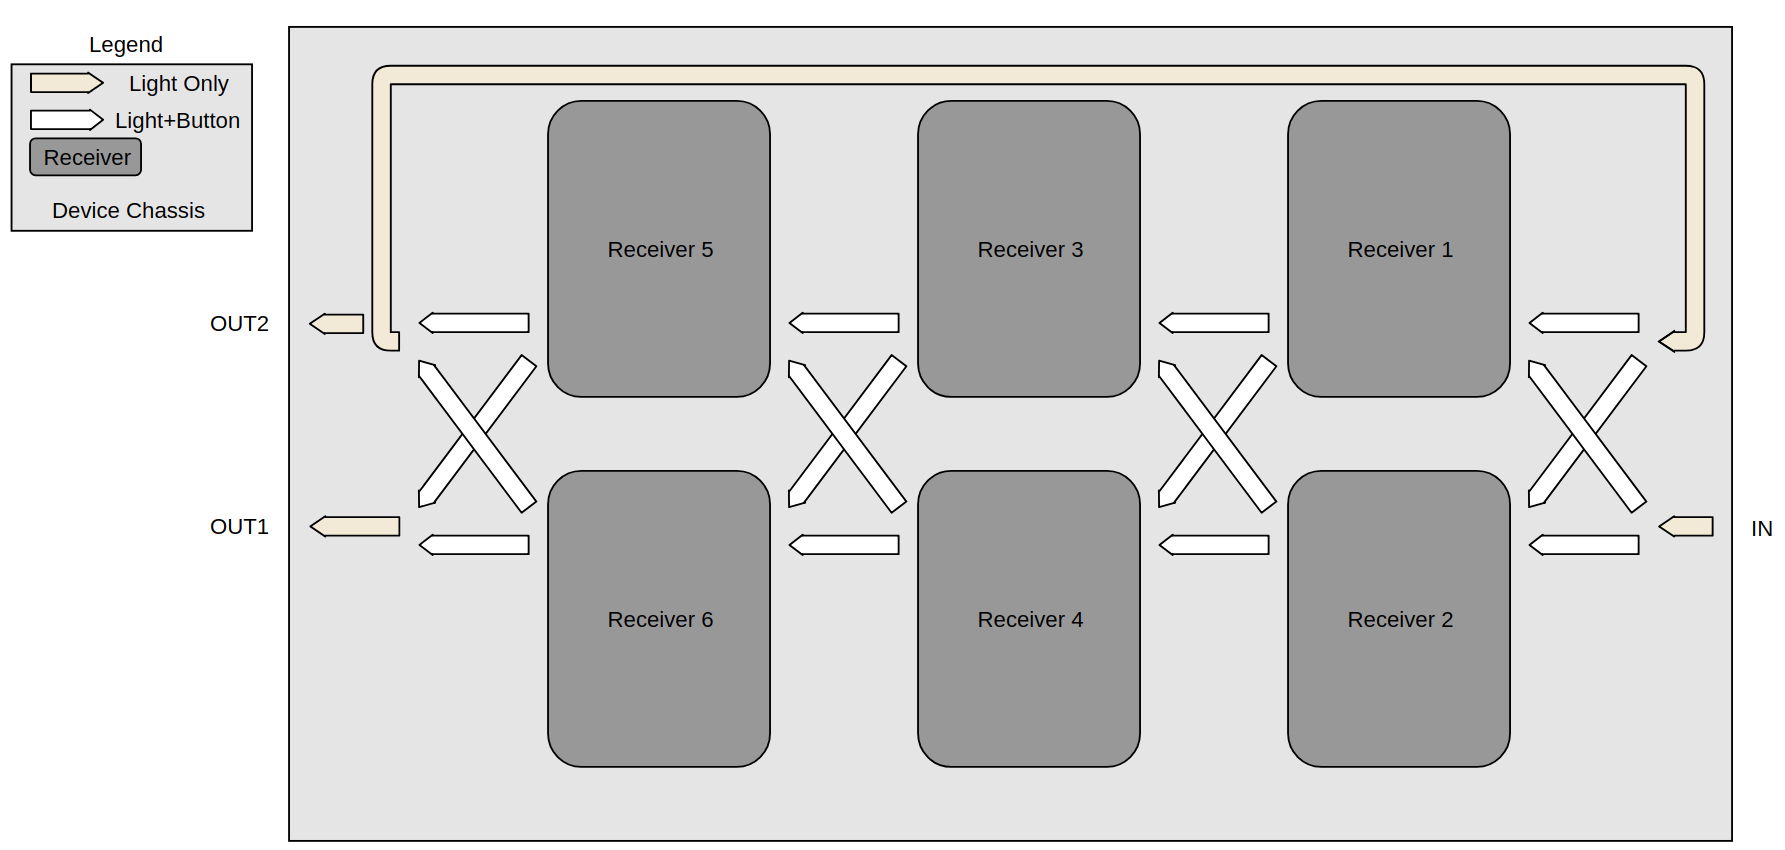
\includegraphics[width = \textwidth]{PR4Images/UIOverview.png}
		\caption{Overview of the user interface for understanding the physical layout of the overall unit.}
		\label{fig:OverallUILayout}
	\end{figure}

	To conform with guitar effects industry standards, the signal flow for the overall unit is from right to left.  Between each vertical pair of receivers (such as Receivers 1 and 2 in Figure \ref{fig:OverallUILayout} is a set of four integrated buttons and indicators, shown as white arrows.  Each set of these white arrows is connected to one module board and the board's routing subsystem.  Each button in the set is related to one particular signal routing direction.  For example, the arrow that points left from Receiver 2 to Receiver 4 indicates if the output of Receiver 2 is available on the input of Receiver 4.  In this example, that indicator would be lit if Receiver 4's input was either the output of Receiver 2 or the sum of the outputs of Receiver 1 and Receiver 2.  Each arrow shaped button toggles the state of both its LED and the relays associated with its connection.  In addition, there are a few lights, shown as tan arrows, that do not function as switches, and are lit depending on certain parameters.  For example, the indicators for IN, OUT1, and OUT2 are lit when a cable is plugged into the respective output to show that the connection has been correctly made.  In normal operation at a music store, the output will remain plugged in, so this functions as a de facto ON/OFF indicator.  The large indicator representing the feedback path turns on only when the feedback path is active: at least one of the two white arrows on the far right that point from the end of the feedback indicator into Receiver 1 and Receiver 2 are lit.

	In practice, the button-arrow assembly shown above is replicated several times, with different shaped pieces of acrylic to form the arrows.  These are mounted on a bracket which mechanically aligns the hinges from proper orientation.  This bracket has slots cut for the pushbuttons to be mounted with individual height adjustment so that the feel of the unit can be adjusted during fabrication.  Then the bracket and the pushbutton circuit boards are mounted on a larger base plate that connects the enclosure of the unit.  This is shown in Figure \ref{fig:UIASM}.

	\begin{figure}
		\centering
		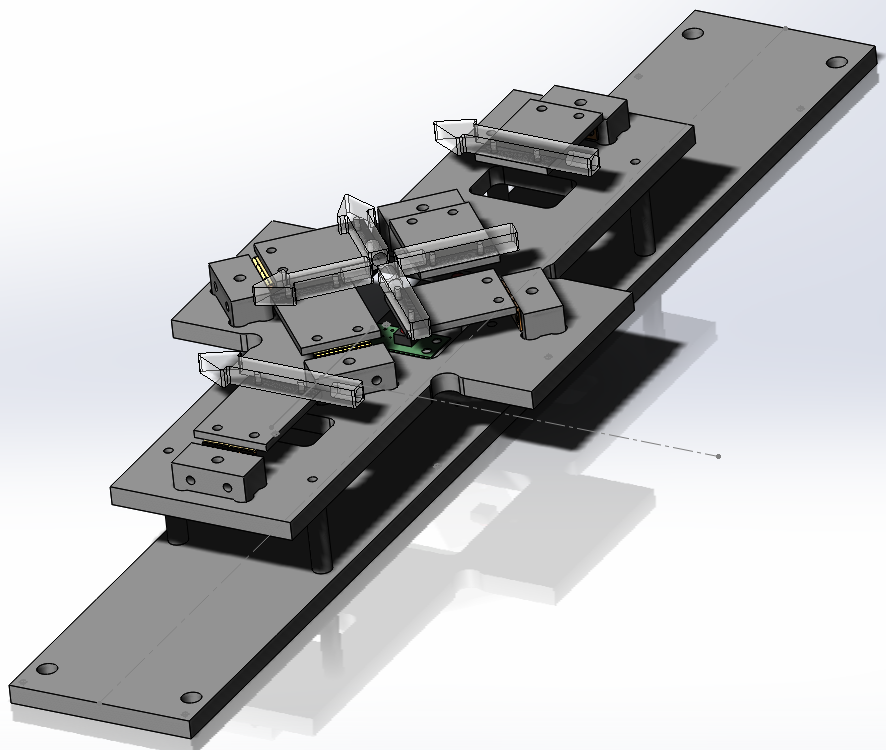
\includegraphics[width = 0.8\textwidth]{PR5Images/UIAsmCAD.png}
		\caption{User Interface subsystem assembly.  This shows the acrylic arrow lights, the circuit boards which hold the pushbuttons, and the assembly plate.}
		\label{fig:UIASM}
	\end{figure}

	\subsubsection{Control Finite State Machine}

	Each routing subsystem is a two input, two output mixer.  Each of the outputs can be the connected to either input or the sum of the inputs.  This means that these outputs can be controlled independently, so each set of white arrows can be split into two groups based on the output they control.  For instance, in Figure \ref{fig:UIarrowlabels}, buttons $a$ and $b$ control the top output while $c$ and $d$ control the bottom output.

	\begin{figure}
		\centering
		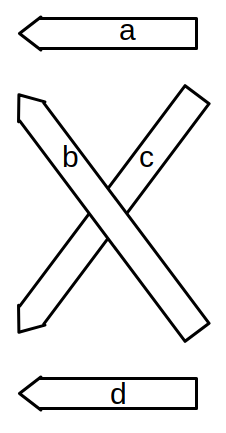
\includegraphics[width = 0.15\textwidth]{PR4Images/UIarrowlabels.png}
		\caption{Set of button-indicators.  These are associated with one module and are used to control the module's signal routing subsystem.  The letters are used for identification in this document.}
		\label{fig:UIarrowlabels}
	\end{figure}

	The switch logic and debouncing is computed on the microcontroller.  The finite state machine depicted in Figure \ref{fig:UIFSM} runs in two instantiations on the microcontroller to cover the $a$ and $b$ set of switches along with the $c$ and $d$ set.  This diagram illustrates only the machine associated with the $a$ and $b$ switches.  This is a Moore state machine where the output is determined by the current state.  The output/state is written in the boxes, and is described by STATE[1:0] where the bit 1 is the state of indicator $a$ and bit 0 is the state of indicator $b$.  The input vector is INPUT[1:0] where bits 1 and 0 represent whether switches $a$ and $b$ are asserted at any given time.

	\begin{figure}
		\centering
		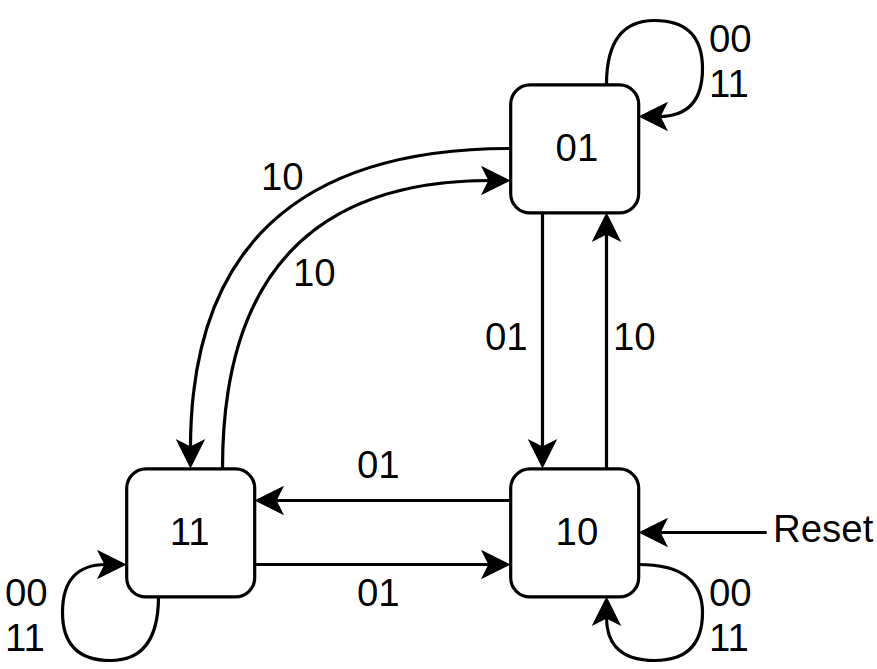
\includegraphics[width = 0.5\textwidth]{PR4Images/UIFSM.png}
		\caption{Finite State Machine describing the operation of the user interface for the signal routing.}
		\label{fig:UIFSM}
	\end{figure}

	As can be seen, the machine always starts in state $\mathtt{10}$, which means that the top input is connected to the top output in a "straight" line.  In terms of Figure \ref{fig:OverallUILayout}, this means that the unit will route the signal

	$$ \text{RECEIVER 1} \rightarrow \text{RECEIVER 3} \rightarrow \text{RECEIVER 5} $$

	This diagram does not indicate any information about the state of the relays in the actual signal routing subsystem.  This is because each FSM state, which is nominally tied to the LED state, also has a dedicated setting for those relays.  All of this information is summarized in a state transition table shown in Table \ref{tab:FSMtransitions}.  Note that state $\mathtt{00}$ should never be reached, as this would indicate that no output is currently selected.  If this state does mistakenly appear, it should transition to state $\mathtt{10}$, which is the default starting state.

	\begin{table}
	\begin{center}
	\begin{tabular}{ |c c|c c|c c|c c|}
	\hline
	\multicolumn{2}{|c|}{State/LED State} & \multicolumn{2}{|c|}{Relay Position} & \multicolumn{2}{|c|}{Input} & \multicolumn{2}{|c|}{Next State} \\
	\hline
	$a(d)$ & $b(c)$ & K1(K4) & K2(K3) & $a(d)$ & $b(c)$ & $a(d)$ & $b(c)$ \\
	\hline
	0 & 0 & 0 & 0 & X & X & 0 & 1 \\
	\hline
	\multirow{3}*{0} 	& \multirow{3}*{1} 	& \multirow{3}*{0} 	& \multirow{3}*{1} 	& 0 & 0 & 1 & 0 \\
						& 					&					&					& 0 & 1 & 1 & 0 \\
						& 					&					&					& 1 & 0 & 1 & 1 \\
						& 					&					&					& 1 & 1 & 0 & 1 \\
	\hline
	\multirow{3}*{1} 	& \multirow{3}*{0} 	& \multirow{3}*{0} 	& \multirow{3}*{0} 	& 0 & 0 & 1 & 0 \\
						& 					&					&					& 0 & 1 & 1 & 1 \\
						& 					&					&					& 1 & 0 & 0 & 1 \\
						& 					&					&					& 1 & 1 & 1 & 0 \\
	\hline
	\multirow{3}*{1} 	& \multirow{3}*{1} 	& \multirow{3}*{1} 	& \multirow{3}*{X} 	& 0 & 0 & 1 & 1 \\
						& 					&					&					& 0 & 1 & 1 & 0 \\
						& 					&					&					& 1 & 0 & 0 & 1 \\
						& 					&					&					& 1 & 1 & 1 & 1 \\
	\hline
	\end{tabular}
	\caption{Routing User Interface FSM transition table.  The table describes the states for the $a$ and $b$ switches, and with the $c$ and $d$ side in parenthesis.}
	\label{tab:FSMtransitions}
	\end{center}
	\end{table}

	The embedded software running on the ATMEGA3209 consists of two of these state machines, as well as two of the state machines that define the receiver operation.

	\subsubsection{Electrical Design}
	The electrical hardware design of the user interface is very simple.  The buttons are connected directly between pins on the ATMEGA3209 and ground, and pull down the inputs when they are activated.  The more interesting facet are the LED drivers.  They use a standard constant current LED driver circuit, controlled from the microcontroller.  Because the ATMEGA3209 has a limited maximum ground current, it cannot be used to drive the LEDs directly.  White LEDs are used for visual effect, and they are typically specified for a forward current of 20mA.  Figure \ref{fig:LEDdriver} shows the circuit.  The LED has a 3V forward voltage drop and should have a 20mA forward current.  This means that the collector voltage of the BJT may be no greater than 2V given the 5V supply.  Choosing an emitter voltage of 1.5V allows for a 500mV drop from the collector to the emitter to allow for variations in LED forward voltage.  R24 is used to set the current given this emitter voltage.  Because the base voltage should be one diode drop above the emitter, the resistive divider formed by R40 and R42 set the base voltage to be 1.9V.  A $\beta$ of 100 suggests that the base current will be 200$\mu$A.  This constant current source should keep the LEDs lit evenly.

	\begin{figure}
		\centering
		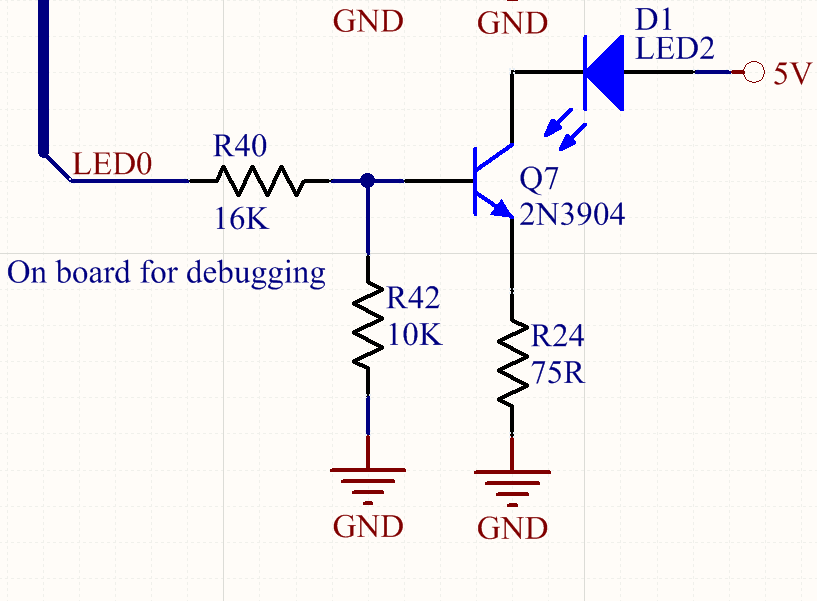
\includegraphics[width = 0.5\textwidth]{PR4Images/LEDconstcurrentdriver.PNG}
		\caption{Constant current source for LED.}
		\label{fig:LEDdriver}
	\end{figure}




